\chapter[Week of Propositional Dynamic Logic]{Program to proof and back again: An introduction to the Propositional Dynamic Logic}

\setcounter{section}{-1}

\section{Heading into next week}

Please read the following article about the Propositional Dynamic Logic. It is from the Stanford Enclyclopedia of Philosophy.
Make as much progress on it as you can. Here is the url for the article: \url{https://plato.stanford.edu/entries/logic-dynamic/}.
If you are interested, the following exercises may help to deepen your understanding.

\begin{enumerate}
    \item Explain why the following gives a program that does ``while $\phi$, do $A$'':  $(\phi ? ; A)^* ; \logicnot \phi ?$ .
    \item Explain why the following gives a program that does ``if $\phi$, then $A$, else $B$'': $(\phi ? ; A) \cup (\logicnot \phi ? ; B)$.
\end{enumerate}

\section{Bonus section: Some PDL humor}

Someone really clever added the following to the wiki page for dynamic logic. Please enjoy.

\begin{center}
    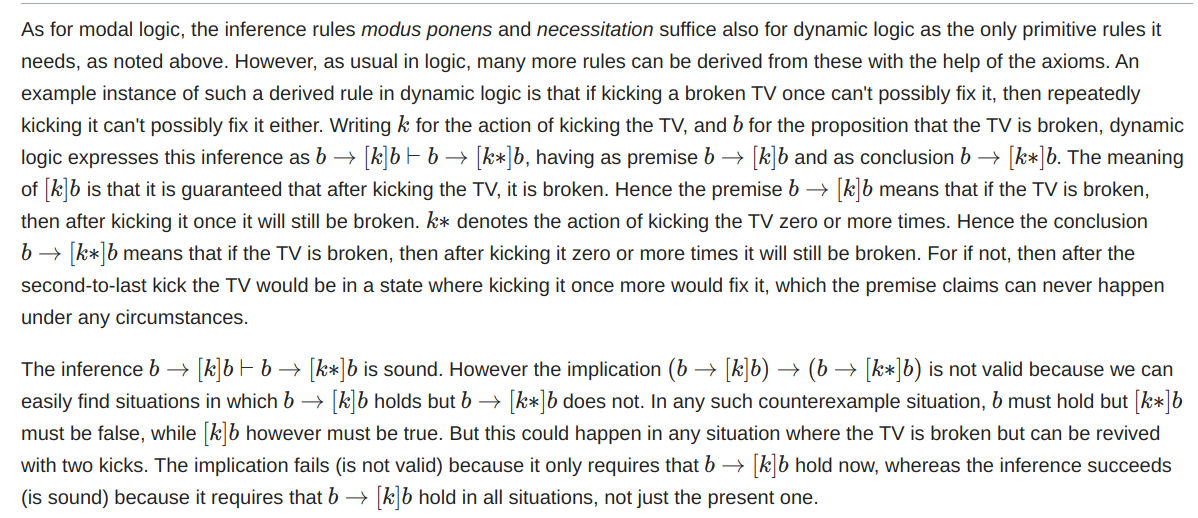
\includegraphics[width=\textwidth]{image (1).png}
\end{center}